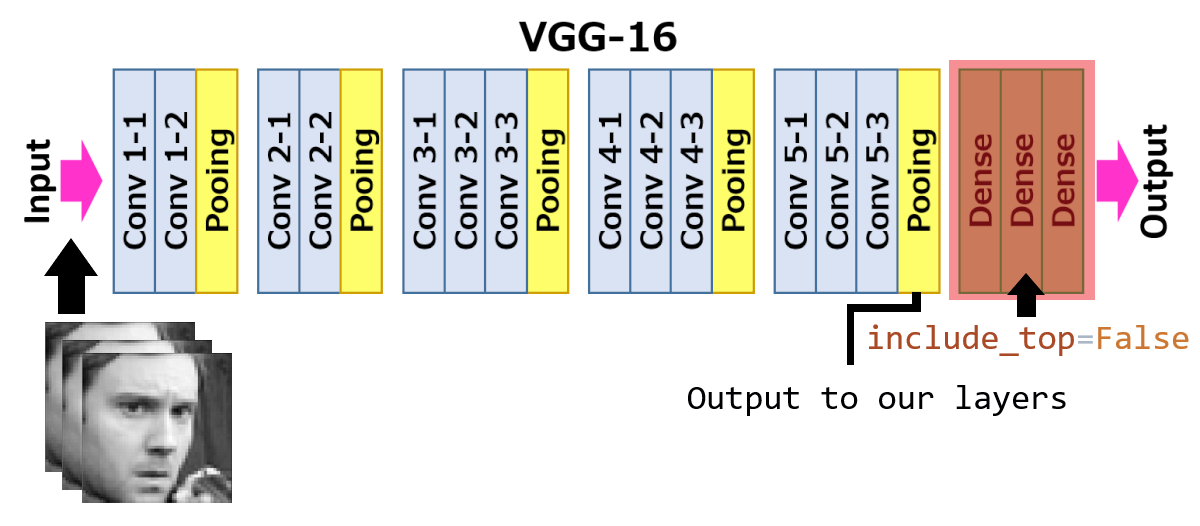
\includegraphics[scale=0.5]{images/modelOne/vgg16layers.png}
At the beginning we have to implement vgg16 model to our environment:
\begin{lstlisting}[language=Python]
    vgg16 = VGG16(include_top=False,
                input_shape=(48, 48, 3),
                pooling='avg',
                weights='imagenet')
\end{lstlisting}

While working at the model we took two approaches:
\begin{itemize}
          \item train whole model with vgg16 frozen layers
          \item get vgg16 output and train our model (final layers) separately
\end{itemize}
First idea took too much time to train, so we decided to get the output of VGG16 and then proceed through our layers and train only a few layers.\\
After that we connect this two models:
VGG16 + our layers.


